\documentclass[12pt]{article}
\usepackage[margin=1in]{geometry}

\usepackage{wrapfig}
\usepackage{graphicx}
\graphicspath{ {figures/} }

\usepackage{enumerate}
\usepackage{enumitem}
\setlist{nolistsep}

\title{Understanding the Clinical Microbiome \\ Biological Engineering Thesis Proposal}

\author{Claire Duvallet}
\date{October 11, 2016}

\begin{document}


\maketitle
\newpage
\tableofcontents

\begin{abstract}
Analyzing the microbiome is hard. Getting clinical insights from analyses is even harder. I'm gonna do some analyses to give us insight into an under-studied clinical microbial system, do some meta-analyses to get direly-needed biological consensus on gut microbiome and disease, and propose a new tool for analyzing 16S datasets.
\end{abstract}
\newpage

\section{Overall objectives and specific aims}
\subsection{Overall objectives}

In spite of the recent increase in research about the human microbiome, there is not a clear consensus on the relationship between human microbial communities and disease. Current 16S microbiome analyses typically study one patient cohort in one disease state, searching for individual disease-associated microbes. However, different published studies for the same disease often contain contradictory or inconsistent results. Existing meta-analyses rarely expand to more than one or two diseases, and thus do not distinguish between microbes which are associated with specific diseases from those which are associated with disease in general. Finally, there are no established tools to extract general biological insights from groups of disease-associated microbes.

This thesis will increase our understanding of the clinical microbiome by moving analyses from focusing on single microbes in individual diseases toward consolidation of groups of related microbes across many different kinds of diseases. In this thesis, I will first apply standard methods to characterize the under-studied microbiota of the aerodigestive tract of one patient cohort. Then, I will perform a comprehensive meta-analysis of gut microbiome studies across many disease states with multiple patient cohorts. Finally, I will develop a tool to enable generalizable interpretation of results from existing and future microbiome studies. This work will improve our understanding of the clinical relevance of the human microbiome and will also provide new approaches and tools for analyzing future studies.

\subsection{Specific Aims}
\begin{description}
	\item[Aim 1] Apply standard methods to identify microbial community characteristics associated with gastro-esophogeal reflux disease and aspiration.
		\begin{enumerate}
			\item Determine how lung, gastric, and throat microbial communities are related.
			\item Identify clinical modulators of lung, gastric, and throat microbial communities.
		\end{enumerate}
	\item[Aim 2] Perform a meta-analysis of case-control gut microbiome studies to identify consistent microbial signatures within and across multiple diseases.
	\begin{enumerate}
		\item Compile and process publicly available case-control gut microbiome studies using a standardized method.
		\item Identify microbes that are consistently associated with specific diseases and with disease in general.
		\item Compare results betweens studies to identify similarities in microbial characteristics of physiologically-related diseases.
	\end{enumerate}
	\item[Aim 3] Enable generalizable interpretations of microbiome analyses by assigning bacteria to groups with similar functions and known associations with disease.
	\begin{enumerate}
	\item Combine existing databases with targeted literature searches to define \textit{microbe sets} based on known biological relationships.
	\item Use machine-learning techniques to extract disease-associated \textit{microbe sets} from datasets collected in Aim 2.
	\item Develop these \textit{microbe sets} into a collaborative tool for use in interpreting new microbiome studies.
	\end{enumerate}
\end{description}
\newpage

\section{Background and significance}
\textit{Three to five pages}

The microbiome is a hot hot hot field and we know some stuff but we don't know a lot of stuff too.

My aims cover multiple body systems: aerodigestive and gut. My aims also span from one study to many, so need to talk about those approaches.

\subsection{Biological background and significance}

\subsubsection{Aerodigestive tract}
The aerodigestive tract consists of the upper gastrointestinal and respiratory tracts (REF). From an engineering perspective, the stomach, throat, and lungs can be thought of as different compartments connected by the esophagus and windpipe. (FIGURE) The mass transport between these compartments is regulated by complex physiological mechanisms. Swallowing guides material from the mouth to the stomach, but may dysfunction and allow material to enter the lungs. The esophageal sphincter usually prevents material from leaving the stomach, but in some diseases is dysfunctional. Finally, complex homeostatic mechanisms clear the lungs of foreign bodies and create a very selective environment for microbes in the lungs (REFS REFS REFS). Thus, while the throat, stomach, and lung "compartments" are physically connected, the amount of material, including bacteria, flowing between them is not readily apparent. 

\subsubsection{Gastro-esophogeal reflux disease and aspiration}

Gastro-esophogeal reflux disease (GERD) is set of syndromes in which the reflux of stomach contents leads to troublesome symptoms or complications (\ref{ref:Vakil}, \ref{ref:dent}) (FIGURE - Figure 2 of Vakil et al). The most common symptoms of GERD are regurgitation and heartburn, but the disease may also present asymptomatically (\ref{ref:Vakil}, \ref{ref:dent}). GERD can be diagnosed by demonstrating reflux of gastric contents (via pH and impedance monitoring), injury to the esophogus (via endoscopy), or based on symptoms alone (\ref{ref:Vakil}). 

Aspiration is the inhalation of foreign material such as food or gastric contents into the lungs \ref{ref:raghavendran}). Most aspiration events are unwitnessed without obvious outward signs or symptoms, and may involved large quantities of aspirated material or may be micro-aspiration events  (\ref{ref:raghavendran}). Aspiration resulting from swallowing dysfunction can be diagnosed with a Modified Barium Swallow test (MBS) (\ref{ref:martin_harris_vfss}). In the MBS procedure, patients are observed videoradiographically as they swallow varying quantities and viscosities of food or liquid impregnated with barium, a contrast agent. The swallowing process is observed and abnormalities like aspiration of contents past the vocal chords can be diagnosed (\ref{ref:martin_harris_clinical_mbs}, \ref{ref:martin_harris_vfss}). However, the MBS test cannot be used to determine aspiration of gastric contents or episodes of micro-aspiration, which may also have clinical relevance (\ref{ref:raghavendran}, \ref{ref:lee}). No validated clinical biomarkers exist to diagnose and define gastric and micro-aspiration events(\ref{ref:lee}), but they are thought to play a role in causing or exacerbating many respiratory diseases (\ref{ref:reen}, \ref{ref:Al-momani}, \ref{ref:raghavendran}, \ref{ref:houghton_2016}). Currently, microaspiration of gastric contents is studied by measuring the concentration of bile or pepsin in the lungs, but such assays are rarely validated against gold-standard methods and have not undergone clinical validation (\ref{ref:houghton_2016}, \ref{ref:lee}). Further complicating the issue is that many healthy patients have a baseline level of micro-aspiration (REF).

\subsubsection{GERD, aspiration, and respiratory disease}
GERD is associated with many respiratory diseases, but the precise link and mechanisms underlying these associations remains very unclear (\ref{ref:houghton_2016}). The prevalence of GERD in respiratory diseases has been estimated to be up to 90\% for some diseases, and often presents without the common symptoms of heartburn or regurgitation (\ref{ref:houghton_2016}). Studies have shown that GERD is related to adverse outcomes after lung transplantation (\ref{ref:Al-momani}) and reduced lung function in patients with cystic fibrosis (\ref{ref:Al-momani}). Aspiration of stomach contents is thought to contribute to these adverse outcomes, either through the aspiration of bile triggering a change in the lung's environment and making it more favorable to colonization, or through direct aspiration of gastric bacteria leading to infection (\ref{ref:Al-momani}, \ref{ref:reen}). However, because of the difficulties in diagnosing and studying microaspiration, aspiration of gastric contents, and GERD, precise causal links between reflux, aspiration, and lung disease have yet to be established (\ref{ref:Al-momani}, \ref{ref:houghton_2016}).

\subsubsection{Microbiome of the aerodigestive tract}
The microbiota of the human lungs and stomachs are among the least well-studied human-associated microbial communities. In fact, the lungs are classically thought to be sterile and free of bacteria in healthy people \ref{ref:charlson-topographical}, \ref{ref:bassis-source}. Neither gastric nor lung sites were included in the Human Microbiome Project, leading to a dearth of studies and data on these important body sites (HMP REF). However, subsequent studies have found suggestions that aerodigestive tract sites are microbially related, and that these microbiomes are altered in certain disease states (REFS).

Only one previous study has examined the relationship between sites of the upper aerodigestive tract (REF). Bassis et al. found that oral microbial communities were more similar to both stomach and lung communities than nasal communities. However, these authors did not examine the inter-relationships between all sites - their driving hypothesis was that the mouth is the source of the downstream communities. In this work, we will take a broader view: which of the upper aerodigestive body sites exchange microbes, are these the same microbes across multiple patients, and are there  patterns for these shared microbes? 

\subsubsection{Lower gastrointestinal tract: physiology and microbiome}
The human gastrointestinal tract is integral to health and disease. Its primary function is to digest food and absorb nutrients, and it also plays important roles in many other aspects of physiology. For example, it is the largest secretor of serotonin and something else (blood flow??) (REF?!). The lower gastrointestinal tract is populated by a complex microbial community, which serves important functions in digesting and salvaging additional nutrients, interacting with the immune system, and protecting the gut from invasion by pathogenic organisms (REF). 

We know that the microbial communities in our guts are unique, modifiable, and integral to our overall health. Studies have consistently shown that gut microbial communities are more similar within a person over time than across people (REF). Environmental disruptions like travel, change in diet, or antibiotics can have both reversible and irreversible changes on the composition of the gut microbiome (REF). Fecal microbiota transplants have demonstrated the causal ability of the microbiome to impact health in both animal models and human patients, and more targeted therapies like narrow-spectrum antibiotics or strain-specific probiotics are an active area of research and development (REF). Experiments with germ-free model organisms have also clearly demonstrated the microbiome's causal role in sustaining health and causing disease (REF).

\subsubsection{Microbiome/disease associations of the lower gastrointestinal tract}
Because of the microbiota's importance in the healthy function of the gastrointestinal tract, associations between microbial communities have been investigated for a wide variety of diseases (REFS). 

Because of its important role in human physiology, many disorders are related to a dysfunctional intestinal tract. Metabolic syndromes like obesity and diabetes 

\subsection{Analytical background and significance}

\subsubsection{Data generation and challenges}
The advent of high throughput next generation sequencing has enabled culture-independent analyses of complex microbial communities. Briefly, DNA is extracted from biological samples of interest and a portion of the universal bacterial 16S region is amplified. Data is sequenced using a variety of available technologies, usually with 454 Pyrosequencing or, more recently, Illumina HiSeq or MiSeq (REFS). The resulting reads are quality-controlled and processed into Operational Taxonomic Units (OTUs), clusters of similar sequences which serve as proxies for bacterial species. OTUs can be assigned bacterial taxonomies using a variety of methods, for example by mapping them to annotated reference genomes or using Bayesian inference trained on a reference set of annotated bacteria (GG and RDP REFS). 

The resulting datasets are often very high-dimensional, with hundreds of OTUs present in a given cohort which may only have tens of samples. The data is also incredibly sparse: only very few OTUs tend to be present in many of the samples, and most entries in the data matrix are zeros. Furthermore, technical artifacts such as DNA extraction and PCR amplification biases are known issues that lead to strong batch effects across different studies. Different data processing, quality filtering, and name-assignment methods also lead to strong batch effects. For example, different taxonomy databases contain different microbes or conflicting names for the same bacteria, making it difficult to compare even published, annotated results across studies.  These issues are major contributors to the lack of consensus on the role of the microbiome in disease, in spite of the availability of many studies.

\subsubsection{Current analytical approaches for 16S analyses}
Including how community related-ness is measured.

Common methods: Alpha diversity, JSD, t-tests, etc
Data analysis: lots of multiple corrections to do

Data processing: different methods (OTU calling, Latin name mapping) lead to drastically different results

What studies exist, sample size limitations, different technologies, batch effects.

\subsubsection{Existing meta-analyses}
Haven't found much and haven't been great.

\subsubsection{Databases and tools for annotations}
GSEA is commonly used in RNAseq data! Gene databases exist and have been curated into gene sets.
No curated microbe sets. Some existing similar tools: SourceTracker, ImG, ...?

\section{Research design and methods}
\textit{Six to eight pages}

\subsection{Aim 1: Aerodigestive microbiota associated with GERD and aspiration}

\begin{wraptable}{r}{5.5cm}
\begin{tabular}{|l|c|}
	\hline
	\textbf{Sites} & \textbf{N} \\
	\hline
	gastric, throat, \& BAL & 87 \\
	gastric \& throat & 45 \\
	gastric \& BAL & 34 \\
	BAL \& throat & 9 \\
	\hline 
\end{tabular}
\caption{Aerodigestive site samples}\label{tab:rosen_samples}
\end{wraptable}

As discussed previously, patients with aerodigestive disorders like aspiration and GERD are at a higher risk for respiratory infections. We hypothesize that microbial communities in the aerodigestive tract share and exchange certain members which then contribute to infections, and that clinical factors like reflux or aspiration disease change the amount of bacterial exchange between aerodigestive sites.

Our patient cohort consists of 261 patients recruited by Rachel Rosen (M.D., GI/Nutrition) at Boston Children's Hospital for multiple studies over the course of the past 6 years. Multiple samples were taken from patients: throat swabs, gastric fluid, and broncho-alveolar lavages (BAL) (Table \ref{tab:rosen_samples}). 125 patients were monitored for full-column GERD and 112 patients were tested for aspiration. Overall, this cohort represents the largest existing human aerodigestive microbiome dataset.


\subsubsection{Exchange of microbes between lung, gastric, and throat communities} \label{sec:exchange}
To understand the microbial exchange between sites in the aerodigestive tract, we will first define a metric to quantify how "shared" microbes are between two sites. There are multiple ways to define this metric: as the percentage of patients who have the microbe present in both sites, as the correlation between the abundance of the microbe in one site with its abundance in the other site, or some combination of these two approaches. Because many microbes in the stomach and lungs are seeded by the oral community, simple co-occurence of bacteria is not sufficient to establish meaningful microbial exchange (REF). Using the correlation of abundances in two sites is also not adequate, since many people may not have the OTU present in either or both sites due to the inherent variability of microbial communities between people.

Thus, we will use both co-occurence and correlation to quantify microbial exchange across sites, which we call $p_s$. We will first identify which microbes are shared using the abundance correlation, and then quantify each microbe's degree of sharedness by its co-occurence rate in patients. For each microbe, we will calculate the non-parametric Spearman rank correlation of the log10(relative abundances) in the two sites, using only abundances from patients with the microbe present in both sites. If this correlation is greater than 0.5, the microbe is considered to be shared. Our metric $p_s$ is then defined as the percentage of patients who have the microbe present in both sites (Fig. \ref{fig:sharedness_defn}).

\begin{wrapfigure}{R}{0.5\textwidth}
	\centering
    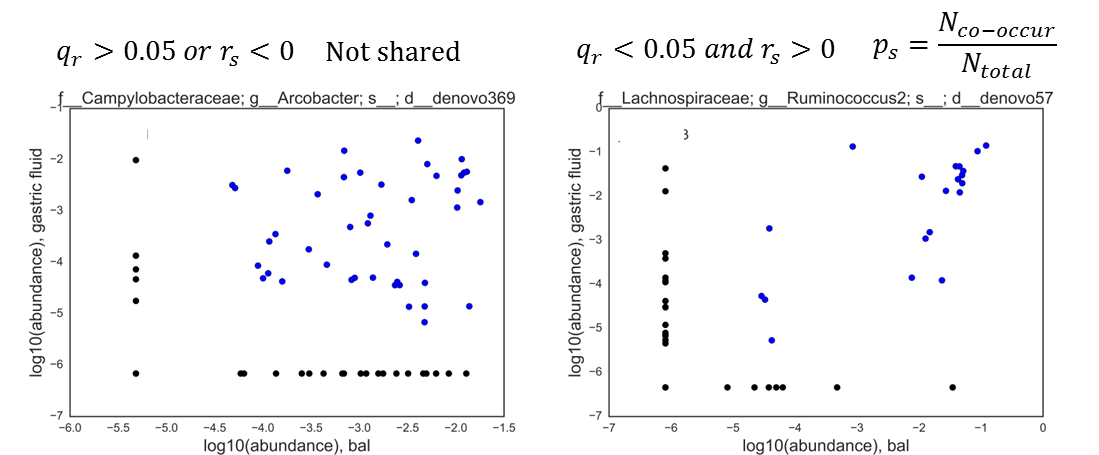
\includegraphics[scale=0.5]{sharedness_definition}
    \caption{Determining $p_s$}\label{fig:sharedness_defn}
\end{wrapfigure}


\subsubsection{Clinical modulators of lung, gastric, and throat microbial communities}
Once we quantify microbial exchange within the aerodigestive tract, we can begin to ask which clinical factors modulate how much exchange occurs between sites. We will calculate $p_s$ for all a-priori defined exchanged microbes (Section \ref{sec:exchange}), stratified by the clinical factor. Furthermore, we will investigate whether the total abundance of exchanged microbes in the different sites and beta diversity community similarities differ between our case and control patient groups.

Our first hypothesis is that aspirators will have a stronger connection between their throat and lungs. Additionally, because many of these patients have GERD, we also expect a slight increase in the connection between the stomach and lungs. Our dataset has 48 patients with abnormal MBS test results (Aspirators) and 63 patients with normal results.

Our next hypothesis is that patients with more severe GERD will have more sharing between the stomach and lung communities. Because are interested in GERD that may modulate the stomach-lung connection, we define "severe GERD" as reflux in which more than 50\% of events are full-column reflux events. With this definition, we have 99 patients with severe GERD and 26 patients without. In addition to the binary severe/not severe comparison, we may regress each of the continuous measures of GERD severity onto the abundance of microbes in each patient's lung and stomach communities. We will also investigate how PPIs modulate the connection between aerodigestive sites, since PPIs are often prescribed for respiratory disease but have unclear clinical impact. The dataset has 114 patients on PPIs and 85 patients not on PPIs.

\subsubsection{Additional considerations}
One factor to consider when drawing conclusions from the $p_s$ metric is that because of the low bacterial biomass in the gastric and lung sites, it is possible that some microbes which are "exchanged" across these sites are simply both being seeded by the environment. However, if these microbes are phylogenetically related or they are known members of the gastric or lung communities, this would indicate that the OTUs are being selected for by the environment and are relevant community members.

This work does not address the direction of microbial exchange between aerodigestive sites, nor does it directly link increased microbial exchange with adverse outcomes like respiratory infections. Follow up studies focus on patients who develop respiratory infections, or patients who frequently have GERD- or aspiration-associated respiratory infections. 

Finally, an important caveat to note when discussing the human lung and gastric microbiomes in general is that our basic understanding of these communities in healthy humans is still quite rudimentary. For example, the extent to which lung microbial communities are composed of surviving and replicating microbes versus transient members is unknown. However, because we do see similarities in microbiota across patients, we can conclude that at least some selection is happening in these sites, and even if these communities are not thriving they may still be physiologically relevant.

\subsection{Aim 2: Meta-analysis of gut microbiome studies}\label{sec:aim2}
By combining results from existing gut microbiome case-control studies, we can move the field toward a consolidated understanding of consistent microbial markers of gut-related diseases. We hypothesize that certain bacteria will often be associated with disease, and that some of these bacteria will be associated with many different types of diseases while others will be unique to one or two conditions. Additionally, we hypothesize that microbial signatures  of health and disease will be more similar in similar diseases (i.e. diabetes and obesity).

\subsubsection{Compile and process gut microbiome datasets}
To perform a comprehensive meta-analysis, we need to collect a comprehensive selection of 16S gut microbiome case-control studies. We will identify these studies through a targeted literature search.  See TABLE for exclusion and inclusion criteria for studies to be considered.

We will process these datasets using a standardized in-house pipeline developed by Thomas Gurry and to which I have contributed. We will start with the rawest available data - in most cases, these will be fastq files but for some studies we will begin from quality-filtered fasta files. Sequences will be quality and length trimmed, clustered at 100\% similarity, and assigned Latin taxonomic names using the RDP classifier. Samples with fewer than 100 reads will be removed from consideration. OTUs with fewer than 10 reads or which are present in less than 1\% of samples will be removed. More stringent quality filtering may be considered in order to reduce noise in the dataset.

Because studies which sequence different 16S regions will have different sequences corresponding to the same bacteria, we can not used sequence-based open-reference approaches to compare OTUs across studies. After assigning Latin names based on OTUs within each study, we will collapse OTUs to the genus level and compare these across studies.

\subsubsection{Identify microbes consistently associated with diseases}\label{sec:indep_studies}
Once we have processed all datasets in a standardized way, our first goal is to identify consistent markers of health and disease. We will analyze each dataset with microbiome methods commonly used in the literature: univariate non-parameteric statistical tests on relative abundances, alpha and beta diversity in different types of patients, and ratios of Firmicutes to Bacteroides in healthy vs. disease patients. It is generally thought that low alpha diversity is a marker of dysbiosis (REF), and that while most people have a Firmicutes/Bacteroides ratio of (XXX), in certain diseases this ratio may be different (REF). (MAYBE BACKGROUND?) By analyzing each study in the same way from raw data, we can reduce the study-wise batch effects and increase our ability to identify general trends in the gut microbiome in health and disease. We will identify consistent markers of disease by using standard meta-analysis methods, comparing the effect sizes and directionality of bacteria across studies, and using Fisher's method to determine overall significant of a microbe (REFS). 

\subsubsection{Compare results between studies for related diseases}\label{sec:signatures}
Our next hypothesis is that similar diseases will have similar signatures of dysbiosis. For example, we expect that metabolic diseases like obesity and diabetes will have more similar microbiota changes than they will to diarrheal diseases like Clostridium difficile infection or enteric diarrhea. We will summarize each dataset with one vector indicating its "microbial signature". This signature will be based on number and identities of microbes significantly associated with the disease and the direction of change of these microbes. Depending on the results from Section \ref{sec:indep_studies}, we may also include factors like differences in alpha diversity or Bacteroides/Firmicutes ratios. Then, we will investigate which datasets cluster together in this "signature space". (Fig. \ref{fig:microbe_signatures})

%\begin{wrapfigure}{R}{0.5\textwidth}
%	\centering
\begin{figure}
\begin{center}
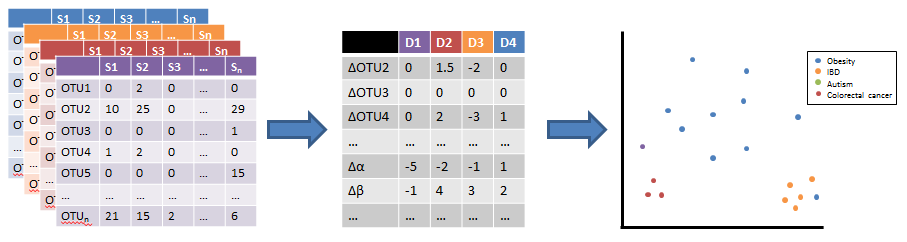
\includegraphics[scale=0.5]{microbial_signatures}
\caption{Defining microbial signatures}\label{fig:microbe_signatures}
\end{center}
\end{figure}
%    \caption{Defining microbial signatures}
%\label{fig:microbe_signatures}
%\end{wrapfigure}


If a disease has a strong impact on or association with the gut microbiome, then we would expect its signatures from multiple studies to cluster very tightly together. If this is the case, we can extract the bacterial features which contribute the most to this tight clustering - these will then be most likely to be associated with that specific disease, and would be good candidates for further mechanistic explorations. On the other hand, if datasets of the same disease or similar conditions do not have similar microbial signatures, this may indicate that the microbiome is not inherently implicated or affected by the disease. In this case, any signal that we see in the gut microbiome is likely driven by other non-disease effects, which are not necessarily the same across studies. Finally, if we find different diseases with similar underlying causes (i.e. inflammation) clustering near each other, then perhaps this would indicate that the microbiome is affected or involved with the underlying cause rather than the specific diseases. Such insights could help us design better experiments to follow up on mechanism or causal relationships.

\subsubsection{Additional considerations}
It is possible that we struggle to find bacteria consistently associated with diseases because of technical batch effects, even where we expect to find a clear signal (i.e. in diseases which have had clear results from experimental or mechanistic studies (REFS)). Developing robust methods to overcome technical batch effects in 16S studies is not within the scope of this work. However, if standard meta-analysis methods fail, we can try some naive correction methods like a linear correction for the principal components which correlate closely with technical artifacts like read depth (FIGURE?). We could also consider using a phylogenetics-based approach rather than taxonomically-assigned closed-reference OTUs. We could identify associations with disease using open-referenced OTUs and then compare their phylogenetic relationships across all studies. Finally, we could also use tools like PiCRUST to assign functionality to our observed taxonomies, and approach our meta-analysis from a functional point of view (REF). 

\subsection{Aim 3: Assigning bacteria to groups with similar functions and disease associations}
Few analytical tools exist to motivate biological hypotheses from the results of high-throughput case-control microbiome studies. Although studies often yield some significant OTU-disease associations, assigning biological interpretations to such results remains challenging. For example, the importance of short-chain fatty acid producers is well-accepted in IBD, and may play in a role in many other diseases as well (REFS). However, directly identifying enrichment functionally-related bacteria (such as SCFA-producing bacteria) is not currently possible. Instead, researchers face the task of interpreting lists of individual OTUs into common biological themes or functions on their own (GSEA REF). 

In this aim, we will curate biologically-motivated \textit{microbe sets} to enable easier interpretation of results from 16S microbiome analyses. By defining groups of related microbes \textit{a priori}, we will enable enrichment analyses similar to GSEA (\ref{sec:something}, REF) for microbiome data. Enrichment analyses will allow for better biological understanding of individual studies' results as well as more consistent comparisons of results across individual studies in the literature.

\subsubsection{Define microbe sets based on known biological relationships}


No existing databases annotate microbes in a way that can be mapped to 16S sequencing studies. Our first task is therefore to curate and define \textit{microbe sets} for use in enrichment analyses of microbiome datasets. We will begin with ImG, an existing database with approximately 10,000 annotated microbial genomes. About half of these genomes are human-associated, and half of those have annotations for categories like disease association, sporulation, body site habitat, and gram staining. We will extract the 16S sequences for all the annotated human-associated microbes in this dataset to determine whether they adequately span the phylogenetic diversity we expect to find in the human gut. If certain key clades are missing from these bacteria, we will manually include them from literature searches and NCBI queries.

In collaboration with Ilana Brito at Cornell, we will apply a combination of literature mining and bioinformatics approaches to fill out the missing annotations in the ImG data and to add our own fields of interest. We will first perform a comprehensive literature review to identify all existing annotated microbial databases. We may also pursue unsupervised text mining of literature results to infer trait-associations for well-studied bacteria (REF). As we populate the microbes in our microbe sets with annotations, we will simultaneously collect their 16S sequences to put them all on a tree. We will apply phylogenetic and phylogenomic inference models to infer the missing traits of leaf organisms when possible.

\begin{table}
\begin{tabular}{|p{6cm}|p{10cm}|}
	\hline
	\textbf{Category} & \textbf{Approach} \\
	\hline
	Pathogens & Targeted literature search, literature mining, \& databases \\
	\hline
	Body sites & Literature mining, machine learning on HMP data \\
	\hline
	Environmental associations & Literature mining, machine learning on EMP data \\
	\hline
	Growth rate & Inference from 16S sequences in datasets from Aim 2 and HMP \\
	\hline
	Obesity-associated & Targeted literature search \& machine learning on Aim 2 datasets \\
	\hline
	Inflammation-associated & Targeted literature search \& machine learning on Aim 2 datasets \\
	\hline
	Miscellaneous functions (acid-tolerant, mucus-degrading, etc) & Targeted literature search, unsupervised PiCRUST clustering \\
	\hline 
\end{tabular}
\caption{Possible approaches to define microbe sets of interest}\label{tab:microbe_set_categories}
%\end{wraptable}
\end{table}


\subsubsection{Extract disease-associated microbe sets from datasets in Aim 2}
We will leverage the datasets collected in Aim 2 to extract additional disease-associated groups of microbes. We will define groups of microbes based on those that distinguished diseases or broader phenotypes in (Section \ref{sec:signatures}). We will also pursue machine-learning driven approaches to identify novel disease- or phenotype-associated \textit{microbe sets}. We will define \textit{microbe sets} based on the most discriminating features of various comparisons, as described in Table \ref{tab:classifications}.

\begin{table}
\begin{center}
\begin{tabular}{|p{6cm}|p{10cm}|}
	\hline
	\textbf{Microbe set association} & \textbf{Classification task} \\
	\hline
	General health/disease & All healthy vs. all disease \\
	\hline
	Diarrhea & CDI, EDD, IBS-D vs. controls \\
	\hline
	Neurological & Autism, Parkinson's vs. controls \\
	\hline
	Immune system & Rheumatoid arthritis, allergy, Crohn's disease, Graft-versus-host disease vs. controls \\
	\hline
	Liver & NASH, MHE (all hepatic diseases) vs. controls\\
	\hline
	Metabolic syndrome & T1D, T2D, obesity, metabolic syndrome vs. controls \\
	\hline
\end{tabular}
\caption{Classification tasks to identify groups of phenotype-associated microbes}\label{tab:classifications}
\end{center}
\end{table}

\subsubsection{Develop collaborative tool for interpreting microbiome studies}
We will make the microbe set annotations available to researchers for further annotation and development. Through our literature searches, we will pay attention to the databases researchers have found most useful and strive to package our annotations in an easy-to-use format. We will likely begin with one very large text file containing all of the microbes, 16S sequences, and metadata that we have gathered. 

We will also package our \textit{microbe set} annotations into a tool that researchers can use to interpret the results of their 16S studies. Our software will take as input an OTU table with taxonomically assigned microbes and disease-state labels for samples. It will perform enrichment analysis on the OTU table and return the results to researchers, similar to the Broad's GSEA tool (REF).

All of this work will be done using public open-source tools like GitHub to encourage collaboration and dissemination of our findings.

\subsubsection{Additional considerations}
Developing a database of microbial annotations is a daunting task due to the vast diversity and complexity of microbes. We recognize the inherent difficulty of this task, and do not expect to produce a fully comprehensive database. However, because our annotations are intended to serve as a tool for biological interpretations and hypothesis generation, even a partially-complete database will be extremely valuable in reducing the number of false-negative results in case-control studies and also providing coherent biological interpretations of existing results. We also recognize that our work will be just the beginning of systematic grouping of phenotypically-associated microbes, and so we will ensure that the format of the database we develop is easily accessible and modifiable by other researchers.

This work will be the beginning of what will hopefully become a new approach to interpreting 16S datasets - moving the field from asking simply "what's different?" toward a more critical interpretation of "why are things different?"

\section{Preliminary studies}
\textit{Three to four pages}

\subsection{Aim 1}
\subsubsection{Microbiome community sharedness}
Look what I can do ma.

\subsubsection{Modulators of sharedness}
And here!

\subsection{Aim 2}
\subsubsection{Collect datasets}
Check out what I got!

\subsubsection{Find consistent microbes}
PCA, alpha diversity, comparing microbial signatures, consistency of significant OTUs.

\section{Gud werds}
We hypothesize that there is a clinically-relevant exchange of bacteria within the aerodigestive tract that may be altered in certain disease states. 


Another important consideration in this work may be if study-associated effects are larger than biological effects. For example, when we compare 'microbial signatures' across datasets, it's possible that the largest signal driving dataset clustering is sequencer or 16S region sequenced, rather than disease state. There are many approaches we could take to correct for such batch effects:
\begin{enumerate}
	\item Subtracting the principal components corresponding to the technical artifacts.
	\item Build a model that accounts for these technical artifacts by including them as factors in the model.
	\item Non-parametric correction, like sample- or OTU-wise quantile normalization, using controls in each study as the reference distribution.
\end{enumerate}

\section{References}
\subsection{Houghton et al}\label{ref:houghton_2016}
Respiratory disease and the  oesophagus: reflux, reflexes and microaspiration
\end{document}

\subsection{Al-momani et al}\label{ref:Al-momani}
Scientific reports, Micoribological profiles of sputum and gastric juice aspirates

\subsection{Reen et al}\label{ref:reen}
Aspirated bile: a major host trigger modulating respiratory pathogen colonisation in CF patients
FJ Reen, DF Woods... F O'Gara

\subsection{Vakil}\label{ref:Vakil}
The Montreal Definition and Classification of Gastroesophageal Reflux Disease: A Global Evidence-Based Consensus
Nimish Vakil, Sander V van Zanten, Peter Kahrilas, John Dent and Roger Jones the Global Consensus Group
http://www.nature.com.libproxy.mit.edu/ajg/journal/v101/n8/full/ajg2006349a.html

\subsection{Dent}\label{ref:dent}
Epidemiology of gastro-oesophageal reflux disease: a systematic review
J Dent1, H B El-Serag2, M-A Wallander3, S Johansson3
http://gut.bmj.com/content/54/5/710.full

\subsection{Lee}\label{ref:lee}
Characteristics and Outcomes of Patients Hospitalized Following Pulmonary Aspiration
Augustine Lee, MD, FCCP,corresponding author Emir Festic, MD, Pauline K. Park, MD, Krishnan Raghavendran, MD, Ousama Dabbagh, MD, FCCP, Adebola Adesanya, MD, FCCP, Ognjen Gajic, MD, FCCP, Raquel R. Bartz, MD, FCCP, and the United States Critical Illness and Injury Trials Group
https://www.ncbi.nlm.nih.gov/pmc/articles/PMC4188146/

\subsection{Martin-harris}\label{ref:martin_harris_vfss}
The Videofluorographic Swallowing Study
Bonnie Martin-Harris, Ph.D., SLP/BRS-Sa,b,c,d and Bronwyn Jones, MB, BS, FRACP, FRCRe,f,g,h,i
http://www.ncbi.nlm.nih.gov/pmc/articles/PMC2586156/

\subsection{Martin-Harris, clinical utility of...}\label{ref:martin_harris_clinical_mbs}
Clinical Utility of the Modified Barium Swallow
Bonnie Martin-Harris, PhD,1,4 Jeri A. Logemann, PhD,2 Steven McMahon, MD,3 Melanie Schleicher, MS,4 and
John Sandidge, MA
\begin{verbatim}http://download.springer.com.libproxy.mit.edu/static/pdf/18/art%253A10.1007%252Fs004550010015.pdf?originUrl=http%3A%2F%2Flink.springer.com%2Farticle%2F10.1007%2Fs004550010015&token2=exp=1473347231~acl=%2Fstatic%2Fpdf%2F18%2Fart%25253A10.1007%25252Fs004550010015.pdf%3ForiginUrl%3Dhttp%253A%252F%252Flink.springer.com%252Farticle%252F10.1007%252Fs004550010015*~hmac=8886a028f336c578123b60769b19c64bb9dfc98f3bc88bac0aa44512d930b77f
\end{verbatim}

\subsection{aspiration induced lung}\label{ref:raghavendran}
Aspiration-Induced lung injury
Krishnan Raghavendran, MD,1 Jean Nemzek, DVM, MS,2 Lena M. Napolitano, MD,1 and Paul R. Knight, MD, PhD3
https://www.ncbi.nlm.nih.gov/pmc/articles/PMC3102154/

\subsection{uppper source of lower and stomach}\label{ref:bassis-source}
Analysis of the upper respiratory tract microbiotas as sorce of lung and gastric
Christine M Bassis, John Erb-DOwnward, et al

\subsection{topographical continuity}\label{ref:charlson-topographical}
topographical continuity of bacterial populations in the healthy respiratory tract